\documentclass[10pt,conference]{IEEEtran}

%%%%%%%%%%%%%%%%%%%%%%%%%%%%%%%%%%%%%%%%%%%%%%%%%%%%%%%%%%%%
%%%%%%%%%%%%%%%%%%%%%%%% PACKAGES %%%%%%%%%%%%%%%%%%%%%%%%%%
%%%%%%%%%%%%%%%%%%%%%%%%%%%%%%%%%%%%%%%%%%%%%%%%%%%%%%%%%%%%

\usepackage{amsmath}
\usepackage{amssymb}
\usepackage{graphicx}
\usepackage{booktabs}
\usepackage{multirow}
\usepackage{algorithm}
\usepackage{algpseudocode}
\usepackage{url}
\usepackage{cite}
\usepackage{array}
\usepackage{float}
\usepackage{subcaption}
\usepackage{xcolor}
\usepackage{enumitem}
\usepackage{bm}
\usepackage{tabularx}
\usepackage{tikz}
\usetikzlibrary{arrows.meta,shapes,fit,backgrounds,positioning,calc}
\graphicspath{{paper/figures/}}

%%%%%%%%%%%%%%%%%%%%%%%%%%%%%%%%%%%%%%%%%%%%%%%%%%%%%%%%%%%%
%%%%%%%%%%%%%%%%%%%%%%%% DOCUMENT %%%%%%%%%%%%%%%%%%%%%%%%%%
%%%%%%%%%%%%%%%%%%%%%%%%%%%%%%%%%%%%%%%%%%%%%%%%%%%%%%%%%%%%

\begin{document}

%%%%%%%%%%%%%%%%%%%%%%%%%%%%%%%%%%%%%%%%%%%%%%%%%%%%%%%%%%%%
%%%%%%%%%%%%%%%%%%%%%%%% TITLE %%%%%%%%%%%%%%%%%%%%%%%%%%%%%
%%%%%%%%%%%%%%%%%%%%%%%%%%%%%%%%%%%%%%%%%%%%%%%%%%%%%%%%%%%%

\title{Knowledge Graph Question Answering Using Reinforcement Learning}

\author{\IEEEauthorblockN{Ankit Rana}
\IEEEauthorblockA{Department of Computer Science and Engineering\\
NIT Calicut}
\and
\IEEEauthorblockN{Dr. Chandramani Chaudhary}
\IEEEauthorblockA{Department of Computer Science and Engineering\\
NIT Calicut}}

\maketitle

%%%%%%%%%%%%%%%%%%%%%%%%%%%%%%%%%%%%%%%%%%%%%%%%%%%%%%%%%%%%
%%%%%%%%%%%%%%%%%%%%%%%% ABSTRACT %%%%%%%%%%%%%%%%%%%%%%%%%%
%%%%%%%%%%%%%%%%%%%%%%%%%%%%%%%%%%%%%%%%%%%%%%%%%%%%%%%%%%%%

\begin{abstract}

% Abstract:
% - Problem
% - Existing limitations
% - Proposed framework
% - Key idea
% - Main results

Multi-hop Knowledge Graph Question Answering (KGQA) demands compositional reasoning over large-scale knowledge graphs. Existing systems rely on static traversal strategies—fixed beam widths, exhaustive expansion—causing excessive exploration and error propagation. RL-based methods improve this but optimize low-level relation IDs, yielding intractably large action spaces and unstable training.

We propose an adaptive neuro-symbolic framework applying RL at two levels: (i) a policy-gradient traversal controller that selects among four high-level width-control actions over a frozen semantic planner, and (ii) a DPO-trained generative judge for preference-aligned candidate selection. We additionally introduce STRL, a curriculum training variant that jointly fine-tunes the planner and controller with InfoNCE semantic supervision.

On ComplexWebQuestions, our primary system (RLMC+DPO) achieves 42.12\% Hit@1 while reducing average expanded graph edges from $>$1,900 to 14 per question—an order-of-magnitude efficiency gain over static traversal—using only RoBERTa-large (355M parameters) without frontier-scale LLMs.

\end{abstract}

\vspace{4pt}\noindent\rule{\columnwidth}{0.4pt}\vspace{2pt}

%%%%%%%%%%%%%%%%%%%%%%%%%%%%%%%%%%%%%%%%%%%%%%%%%%%%%%%%%%%%
%%%%%%%%%%%%%%%%%%%%%%%% KEYWORDS %%%%%%%%%%%%%%%%%%%%%%%%%%
%%%%%%%%%%%%%%%%%%%%%%%%%%%%%%%%%%%%%%%%%%%%%%%%%%%%%%%%%%%%

\begin{IEEEkeywords}
Knowledge Graph Question Answering,
Multi-Hop Reasoning,
Reinforcement Learning,
Neuro-Symbolic Reasoning,
Graph Traversal,
Transformer Models
\end{IEEEkeywords}

%%%%%%%%%%%%%%%%%%%%%%%%%%%%%%%%%%%%%%%%%%%%%%%%%%%%%%%%%%%%
%%%%%%%%%%%%%%%%%%%%%%%% INTRODUCTION %%%%%%%%%%%%%%%%%%%%%%
%%%%%%%%%%%%%%%%%%%%%%%%%%%%%%%%%%%%%%%%%%%%%%%%%%%%%%%%%%%%

\section{Introduction}



Multi-hop KGQA over large knowledge graphs requires compositional reasoning across relational paths, but traversal complexity grows exponentially with depth. Static beam-width strategies over-explore simple questions and under-explore ambiguous ones, while direct RL over raw relation IDs suffers from massive action spaces and unstable optimization.

We propose a three-stage adaptive neuro-symbolic framework. \textbf{Stage~I} (Semantic Planner) learns cross-hop reasoning representations via a transformer planner over RoBERTa-Large. \textbf{Stage~II} (RL Traversal Controller) selects among four high-level width-control actions—\textsc{Tight} ($k$=1), \textsc{Medium} ($k$=5), \textsc{Loose} ($k$=50), \textsc{Stop}—conditioned on frozen planner states, collapsing a $>$10k-relation action space to 4 interpretable decisions. \textbf{Stage~III} (CDS) applies a cascading funnel of bi-encoder, path-aware ranker, and a Flan-T5-Base DPO-aligned generative judge for listwise candidate selection—a second RL-family optimization layer. We additionally propose \textbf{STRL}, a curriculum variant that jointly fine-tunes Stages~I+II with InfoNCE semantic supervision to prevent policy collapse.

On ComplexWebQuestions, our primary system achieves \textbf{42.12\%} Hit@1 while reducing average expanded edges from $>$1,900 to 14 per question, using only RoBERTa-large without frontier-scale LLMs.

%%%%%%%%%%%%%%%%%%%%%%%%%%%%%%%%%%%%%%%%%%%%%%%%%%%%%%%%%%%%
%%%%%%%%%%%%%%%%%%%%%%%% RELATED WORK %%%%%%%%%%%%%%%%%%%%%%
%%%%%%%%%%%%%%%%%%%%%%%%%%%%%%%%%%%%%%%%%%%%%%%%%%%%%%%%%%%%

\section{Related Work}

Knowledge Graph Question Answering (KGQA) has been extensively studied using multiple reasoning paradigms. In this section, we discuss the major categories of existing approaches and their limitations.

\subsection{Semantic Parsing Based KGQA}
Early KGQA systems primarily relied on semantic parsing techniques \cite{yih2015semantic, bao2016constraint} that transformed natural language questions into executable logical forms. While providing strong interpretability, logical form generation often requires expensive annotation and struggles to scale to complex compositional reasoning tasks due to high linguistic ambiguity.

\subsection{Embedding Based KGQA}
Embedding-based methods introduce continuous vector-space representations for entities and relations using techniques such as TransE, DistMult, ComplEx, and RotatE \cite{bordes2013translating, yang2014embedding, trouillon2016complex, sun2019rotate, saxena2020improving, sun2020faithful}. Although these methods improve generalization over purely symbolic approaches, they frequently struggle with long-range relational dependency modeling and lack explicit reasoning transparency because inference occurs implicitly within latent spaces.

\subsection{Graph Neural Network Based KGQA}
Graph Neural Networks (GNNs) \cite{kipf2016semi, velickovic2017graph, schlichtkrull2018modeling, yasunaga2021qa, zhang2022subgraph} model local graph structure using message passing and neighborhood aggregation. While improving structural reasoning, scaling GNNs to deep multi-hop reasoning is computationally expensive, often introducing severe memory overhead and representation oversmoothing as propagation depth increases.

\subsection{Iterative and Reinforcement Learning Based KGQA}
Iterative reasoning systems model KGQA as a sequential traversal process over graph structures \cite{xiong2017deeppath, das2017go, lin2018multi, sun2018open, xian2019reinforcement, sun2019pullnet, wang2020reasoning}. Reinforcement learning (RL) methods further optimize these trajectories by framing reasoning as a Markov Decision Process. However, existing RL-based KGQA systems directly optimize low-level graph actions (e.g., relation IDs or neighboring entities). Consequently, these methods frequently suffer from extremely large action spaces, sparse rewards, unstable optimization behavior, and inefficient graph exploration.

\subsection{Transformer and Structured KGQA}
Recent transformer-based KGQA systems leverage pretrained language models and structured reasoning frameworks \cite{liu2019roberta, jiang2023structgpt, wang2023knowledgpt, luo2024reasoning} to improve semantic reasoning capability and contextual understanding. Despite these improvements, most neuro-symbolic reasoning frameworks still rely on static traversal heuristics during graph exploration and do not dynamically regulate traversal-space expansion according to semantic confidence.

\subsection{LLM-Based KGQA}
Recent literature increasingly emphasizes the use of frontier-scale large language models (LLMs) such as GPT-4 \cite{achiam2023gpt} and Llama \cite{touvron2023llama}, alongside robust conversational and agentic graph reasoning frameworks \cite{christmann2024reign, chen2024spinach, chen2025drkg, zhao2025enrich}. These systems often employ retrieval-augmented reasoning and prompting to navigate symbolic structures. In contrast, the proposed framework prioritizes explicit symbolic traversal and interpretable traversal-control using comparatively lightweight transformer encoders.

Unlike existing methods, our framework decouples semantic reasoning from traversal optimization, enabling efficient and stable adaptive traversal-space control over frozen semantic states.

%%%%%%%%%%%%%%%%%%%%%%%%%%%%%%%%%%%%%%%%%%%%%%%%%%%%%%%%%%%%
%%%%%%%%%%%%%%%%%%%%%%%% PRELIMINARIES %%%%%%%%%%%%%%%%%%%%%
%%%%%%%%%%%%%%%%%%%%%%%%%%%%%%%%%%%%%%%%%%%%%%%%%%%%%%%%%%%%

\section{Preliminaries}

We define the core formalisms used throughout the paper.

\subsection{Knowledge Graph}

A knowledge graph $\mathcal{G}=(\mathcal{E},\mathcal{R},\mathcal{T})$ consists of entity set $\mathcal{E}$, relation set $\mathcal{R}$, and relational triples $\mathcal{T}$. Each triple $(e_s,r,e_o)$ encodes that subject $e_s$ connects to object $e_o$ via relation $r$. The neighborhood of an entity is $\mathcal{N}(e) = \{ e' \mid (e,r,e') \in \mathcal{T} \}$. Real-world KGs such as Freebase contain millions of entities with dense relational structure, yielding large branching factors during traversal.

\subsection{Multi-Hop KGQA}

Given question $q$ and topic entity $e_0$, the task is to retrieve answer set $\mathcal{Y}=\{a_1,\dots,a_n\}$ via sequential traversal $e_0 \xrightarrow{r_1} e_1 \xrightarrow{r_2} \cdots \xrightarrow{r_h} e_h$. At each hop, the candidate set expands as $E_{h+1} = \{ e' \mid (e,r,e') \in \mathcal{T},\, e \in E_h \}$. Traversal-space complexity grows as $\mathcal{O}(b^h)$ where $b$ is the average branching factor, making exhaustive expansion infeasible for deep reasoning chains. Figure~\ref{fig:kg} illustrates a real CWQ multi-hop reasoning trace.

\begin{figure}[!ht]
\centering
\resizebox{\columnwidth}{!}{% ============================================================
%  fig_kg.tex — Complex Multi-Hop Knowledge Graph (Spacious Spread)
%  Shows multiple entities, relation types, branching structure
%  Highlight path: Jerry Jones → Dallas Cowboys → Barry Switzer
% ============================================================

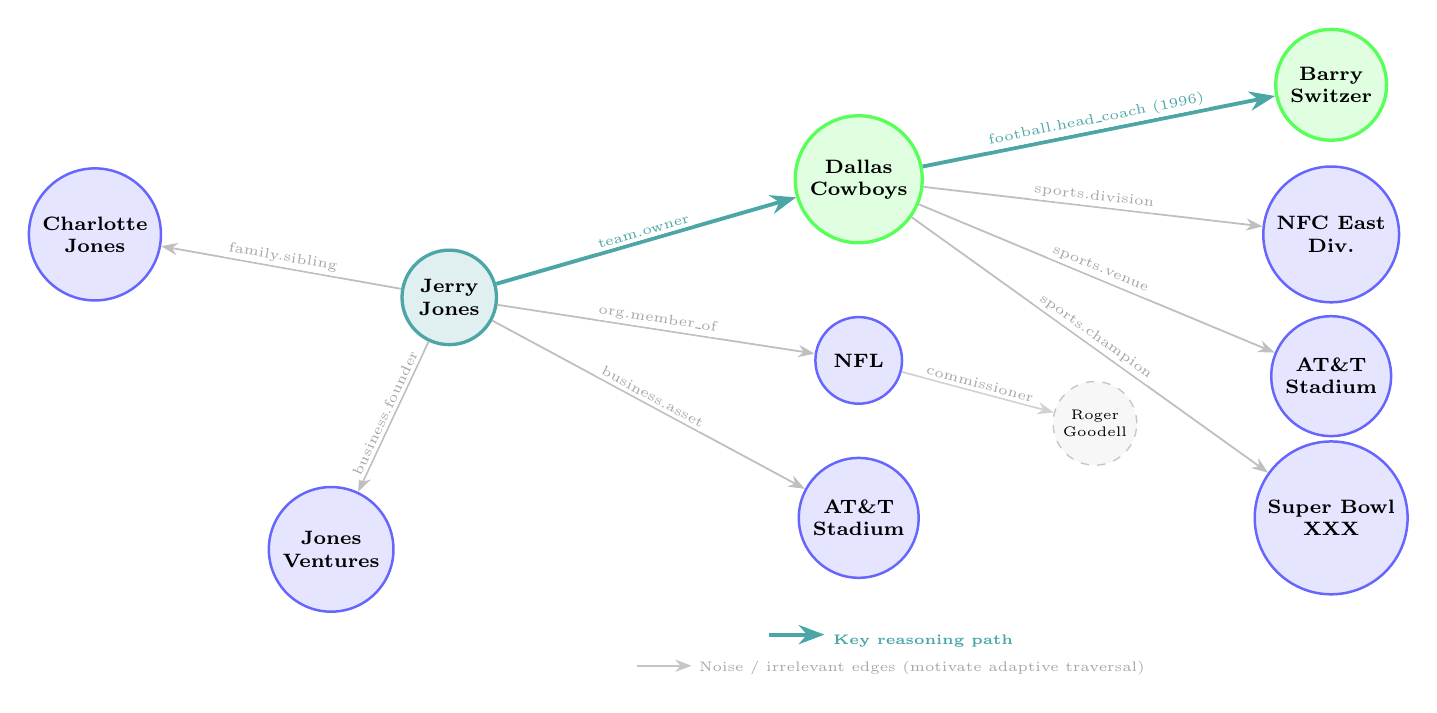
\begin{tikzpicture}[
  font=\small,
  >=Stealth,
  every node/.style={align=center},
  % Entity circles
  entity/.style={
    circle, draw=blue!60, fill=blue!10,
    inner sep=3pt, minimum size=1.1cm,
    font=\scriptsize\bfseries, line width=0.9pt
  },
  centity/.style={
    circle, draw=teal!70, fill=teal!12,
    inner sep=3pt, minimum size=1.2cm,
    font=\scriptsize\bfseries, line width=1.2pt
  },
  aentity/.style={
    circle, draw=green!65, fill=green!12,
    inner sep=3pt, minimum size=1.1cm,
    font=\scriptsize\bfseries, line width=1.2pt
  },
  noise/.style={
    circle, draw=gray!45, fill=gray!6,
    inner sep=2pt, minimum size=0.9cm,
    font=\tiny, line width=0.5pt, dashed
  },
  % Relation edge labels (Centered, sloped, small text)
  rel/.style={font=\tiny, fill=white, inner sep=1.2pt, text=gray!70},
  hrel/.style={font=\tiny, fill=white, inner sep=1.2pt, text=teal!70},
  % Arrows
  earr/.style={->, draw=gray!50, line width=0.65pt},
  harr/.style={->, draw=teal!70, line width=1.4pt},
]

% -------------------------------------------------------
% CENTER — Topic Entity
% -------------------------------------------------------
\node[centity]  (jj)   at (0,0)        {Jerry\\Jones};

% -------------------------------------------------------
% HOP 1 — Direct relations from Jerry Jones (Widely spaced)
% -------------------------------------------------------
\node[aentity]  (dc)   at (5.2, 1.5)   {Dallas\\Cowboys};   % CORRECT PATH
\node[entity]   (nfl)  at (5.2,-0.8)   {NFL};
\node[entity]   (atnt) at (5.2,-2.8)   {AT\&T\\Stadium};
\node[entity]   (biz)  at (-1.5,-3.2)  {Jones\\Ventures};
\node[entity]   (fam)  at (-4.5, 0.8)  {Charlotte\\Jones};

% Hop 1 edges (Sloped, perfectly centered, zero node overlap)
\draw[earr] (jj) -- node[rel,above,sloped,pos=0.5]{org.member\_of} (nfl);
\draw[earr] (jj) -- node[rel,above,sloped,pos=0.5]{business.asset} (atnt);
\draw[earr] (jj) -- node[rel,above,sloped,pos=0.5]{business.founder} (biz);
\draw[earr] (jj) -- node[rel,above,sloped,pos=0.5]{family.sibling} (fam);

% Hop 1 CORRECT edge
\draw[harr] (jj) -- node[hrel,above,sloped,pos=0.5]{team.owner} (dc);

% -------------------------------------------------------
% HOP 2 — Relations from Dallas Cowboys (Widely spaced at x=11.2)
% -------------------------------------------------------
\node[aentity]  (bs)   at (11.2, 2.7)   {Barry\\Switzer};    % ANSWER
\node[entity]   (eag)  at (11.2, 0.8)   {NFC East\\Div.};
\node[entity]   (att2) at (11.2,-1.0)   {AT\&T\\Stadium};
\node[entity]   (sb)   at (11.2,-2.8)   {Super Bowl\\XXX};

\draw[earr] (dc) -- node[rel,above,sloped,pos=0.5]{sports.division} (eag);
\draw[earr] (dc) -- node[rel,above,sloped,pos=0.5]{sports.venue} (att2);
\draw[earr] (dc) -- node[rel,above,sloped,pos=0.5]{sports.champion} (sb);

% Hop 2 CORRECT edge
\draw[harr] (dc) -- node[hrel,above,sloped,pos=0.5]{football.head\_coach (1996)} (bs);

% -------------------------------------------------------
% HOP 2 — Relations from NFL (noise branch)
% Roger Goodell is placed to the right of NFL to avoid AT&T Stadium (at x=5.2)
% -------------------------------------------------------
\node[noise]  (n2)  at (8.2,-1.6)  {Roger\\Goodell};
\draw[earr, draw=gray!35] (nfl) -- node[rel,above,sloped,pos=0.5]{commissioner} (n2);

% -------------------------------------------------------
% LEGEND (Centered at x=5.6)
% -------------------------------------------------------
\node[font=\tiny\bfseries, text=teal!70] at (5.6,-4.3) {%
  \tikz\draw[harr](-0.2,0)--(0.5,0); Key reasoning path};
\node[font=\tiny, text=gray!70] at (5.6,-4.7) {%
  \tikz\draw[earr, gray!45](-0.2,0)--(0.5,0); Noise / irrelevant edges (motivate adaptive traversal)};

\end{tikzpicture}
}
\caption{Multi-hop KG reasoning trace from CWQ. Question: \textit{``Who was the 1996 coach of the team owned by Jerry Jones?''} Teal arrows show the correct 2-hop path: \textit{team.owner} $\to$ Dallas Cowboys $\to$ \textit{football.hist\_coach} $\to$ Barry Switzer. Grey dashed nodes/edges are noise neighbours that static traversal must explore, motivating adaptive traversal-control.}
\label{fig:kg}
\end{figure}


%%%%%%%%%%%%%%%%%%%%%%%%%%%%%%%%%%%%%%%%%%%%%%%%%%%%%%%%%%%%
%%%%%%%%%%%%%%%%%%%%%%%% PROBLEM FORMULATION %%%%%%%%%%%%%%%
%%%%%%%%%%%%%%%%%%%%%%%%%%%%%%%%%%%%%%%%%%%%%%%%%%%%%%%%%%%%

\section{Problem Formulation}
\label{sec:probform}

Static traversal strategies apply identical expansion behavior to all questions regardless of semantic complexity, causing over-exploration on simple queries and under-exploration on ambiguous ones. We formulate traversal-space control as a Markov Decision Process $\mathcal{M}=(\mathcal{S},\mathcal{A},\mathcal{P},\mathcal{F})$, where states $s_t$ are latent semantic representations produced by the planner and actions regulate graph expansion width. The compact action space $\mathcal{A} = \{ a_{\text{tight}},\, a_{\text{medium}},\, a_{\text{loose}},\, a_{\text{stop}} \}$ provides four search-width controls: during training, $a_{\text{tight}}$ restricts traversal to the top-1 relation (beam\,=\,1), $a_{\text{medium}}$ expands to top-5 (beam\,=\,5), and $a_{\text{loose}}$ performs domain-guided search (beam\,=\,50); at inference, beam widths are widened to $\{5, 10, 50\}$ respectively to improve recall at the cost of a noisier candidate pool that the CDS reranker subsequently filters. $a_{\text{stop}}$ terminates the path. Adaptive control reduces traversal complexity from $\mathcal{O}(b^{H_{\max}})$ to $\mathcal{O}(k^{H_{\max}})$ where $k \ll b$. At each step the policy $\pi(a_t|s_t)$ selects a traversal action based on semantic confidence. The step-level reward combines a semantic alignment signal with efficiency and grounding components:

\begin{equation}
\label{eq:reward}
R_t = \alpha\, R^{\text{sem}}_t + \beta\, R^{\text{conn}}_t + \gamma\, R^{\text{eff}}_t + R^{\text{entity}}_t + R^{\text{cur}}_t
\end{equation}

where $R^{\text{sem}}_t$ is the maximum cosine similarity between the hop representation and the top-$k$ relation embeddings within the chosen beam, $R^{\text{conn}}_t$ is a connectivity proxy that thresholds the semantic score ($+0.3$ if best similarity $\ge 0.3$, else $-0.5$), $R^{\text{eff}}_t$ penalises wide actions (Tight $+0.3$, Medium $0.0$, Loose $-0.3$), $R^{\text{entity}}_t$ is a KG-anchored grounding bonus at hop~0 ($+0.6$ if the chosen beam intersects relations reachable from the topic entity, $-0.4$ otherwise), and $R^{\text{cur}}_t$ is a weak curriculum bonus ($+0.2$) during early training epochs when the gold relation appears in the beam. Coefficients: $\alpha{=}0.5$, $\beta{=}0.3$, $\gamma{=}0.2$. This step-level reward $R_t$ is fed back to the reinforcement learning agent at each hop and serves as the optimization signal for policy gradient updates (as detailed in §\ref{sec:stage2_training}). Operating over four high-level actions rather than raw relation IDs keeps the policy space compact and optimization stable.

%%%%%%%%%%%%%%%%%%%%%%%%%%%%%%%%%%%%%%%%%%%%%%%%%%%%%%%%%%%%
%%%%%%%%%%%%%%%%%%%%%%%% METHODOLOGY %%%%%%%%%%%%%%%%%%%%%%%
%%%%%%%%%%%%%%%%%%%%%%%%%%%%%%%%%%%%%%%%%%%%%%%%%%%%%%%%%%%%

\section{Methodology}

The proposed Reinforcement Learning based Meta-Constraint (RLMC) framework addresses multi-hop KGQA through three sequential stages trained progressively. \textbf{Stage~I} (Semantic Reasoning Planner) learns semantic reasoning representations from question-path supervision. \textbf{Stage~II} (RL-Based Traversal Controller) learns adaptive traversal policies via policy gradient optimization over frozen Stage~I representations. \textbf{Stage~III} (Candidate Disambiguation \& Selection, CDS) applies a three-sub-stage cascading funnel—culminating in a preference-aligned generative judge—to select the final answer. We additionally introduce \textbf{STRL} (Semantic-Teacher Reinforcement Learning), an enhanced training variant for Stages~I+II that incorporates a semantic teacher curriculum via InfoNCE contrastive supervision. Figure~\ref{fig:arch} shows the overall architecture.

\begin{figure*}[!t]
\centering
% =====================================================================
%  fig_detailed_dataflow.tex — End-to-End Hierarchical KGQA Dataflow
% =====================================================================

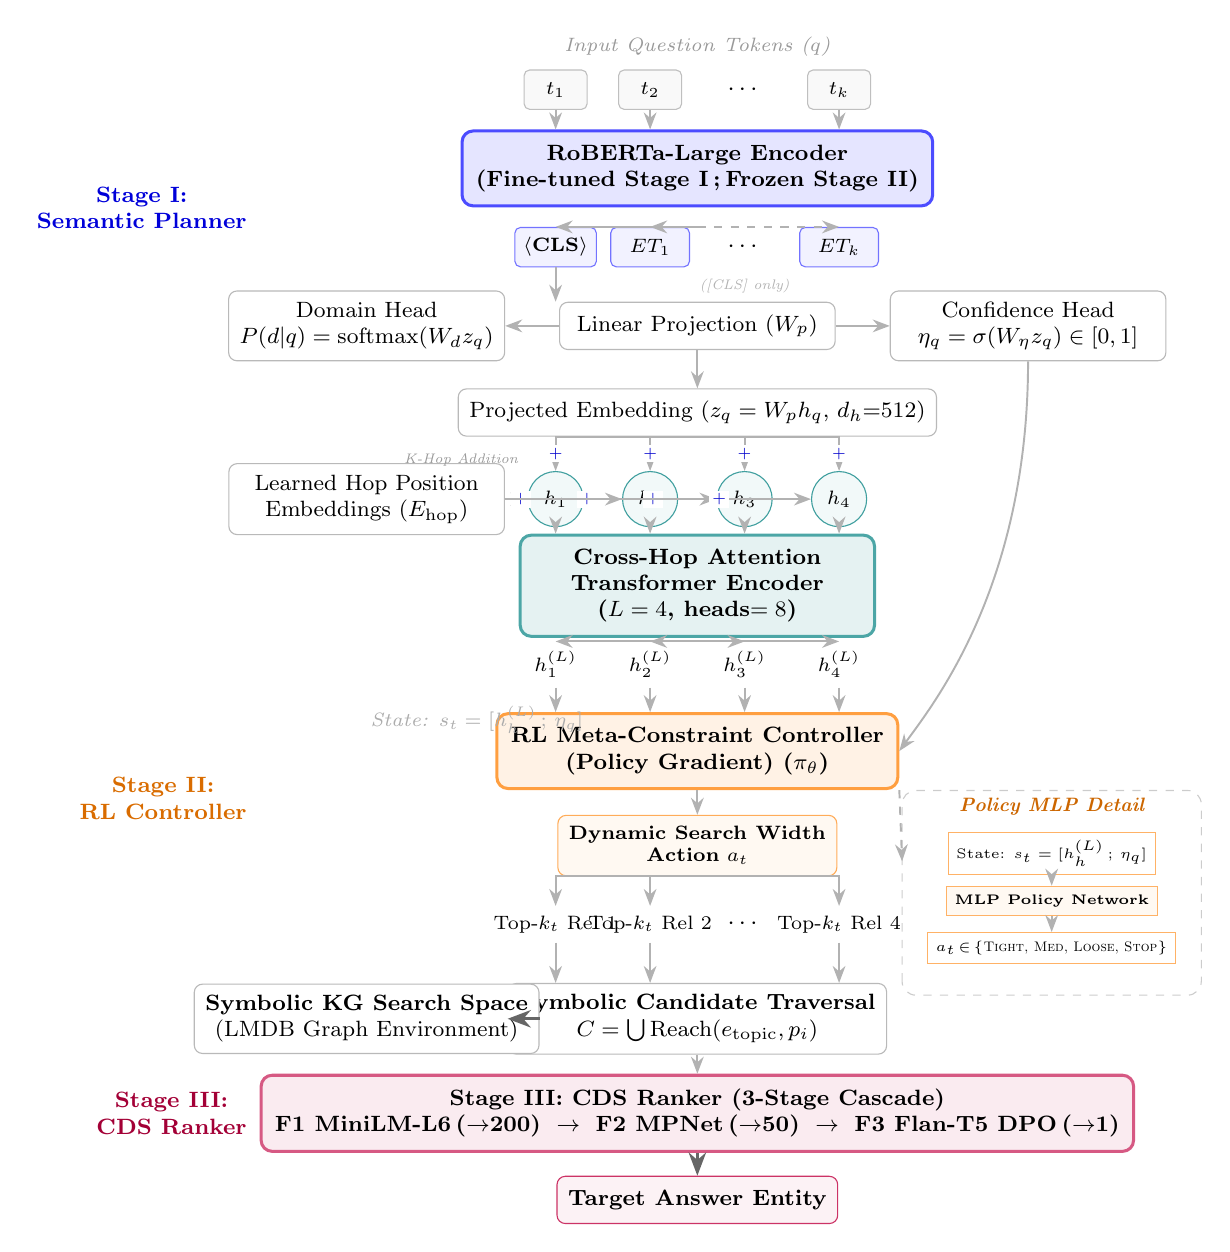
\begin{tikzpicture}[
  font=\small,
  >=Stealth,
  every node/.style={align=center},
  % ---- box styles ----
  tokenbox/.style={
    rectangle, rounded corners=2pt,
    draw=gray!50, fill=gray!5,
    inner sep=3pt, minimum width=0.8cm, minimum height=0.5cm,
    font=\scriptsize
  },
  embbox/.style={
    rectangle, rounded corners=2pt,
    draw=blue!55, fill=blue!5,
    inner sep=3pt, minimum width=1.0cm, minimum height=0.5cm,
    font=\scriptsize\bfseries
  },
  bluebox/.style={
    rectangle, rounded corners=4pt,
    draw=blue!70, fill=blue!10,
    inner sep=5pt, minimum width=4.5cm, minimum height=0.7cm,
    line width=1.1pt, font=\footnotesize\bfseries
  },
  qbox/.style={
    rectangle, rounded corners=3pt,
    draw=gray!55, fill=white,
    inner sep=4pt, minimum width=3.5cm, minimum height=0.6cm,
    font=\footnotesize
  },
  tealbox/.style={
    rectangle, rounded corners=4pt,
    draw=teal!70, fill=teal!10,
    inner sep=5pt, minimum width=4.5cm, minimum height=0.7cm,
    line width=1.1pt, font=\footnotesize\bfseries
  },
  ppobox/.style={
    rectangle, rounded corners=4pt,
    draw=orange!75, fill=orange!10,
    inner sep=5pt, minimum width=4.5cm, minimum height=0.7cm,
    line width=1.1pt, font=\footnotesize\bfseries
  },
  cdsbox/.style={
    rectangle, rounded corners=4pt,
    draw=purple!65, fill=purple!8,
    inner sep=5pt, minimum width=4.5cm, minimum height=0.7cm,
    line width=1.1pt, font=\footnotesize\bfseries
  },
  circlehop/.style={
    circle, draw=teal!75, fill=teal!5,
    inner sep=2pt, minimum size=0.7cm,
    font=\scriptsize\bfseries
  },
  actbox/.style={
    rectangle, rounded corners=3pt,
    draw=orange!65, fill=orange!5,
    inner sep=4pt, minimum width=3.5cm, minimum height=0.6cm,
    font=\scriptsize
  },
  arr/.style={->, draw=gray!60, line width=0.7pt},
  Arr/.style={->, draw=black!60, line width=1.2pt},
  dashedarr/.style={->, draw=gray!60, dashed, line width=0.7pt},
]

% ══════════════════════════════════════════════════════
% STAGE I — Semantic Planner (Top Block)
% ══════════════════════════════════════════════════════

% 1. Input Question Tokens
\node[tokenbox] (t1)   at (-1.8, 2.8) {$t_1$};
\node[tokenbox] (t2)   at (-0.6, 2.8) {$t_2$};
\node           (dots) at (0.6,  2.8)  {$\cdots$};
\node[tokenbox] (tk)   at (1.8,  2.8) {$t_k$};
\node[anchor=south, font=\scriptsize\itshape, text=gray!80] at (0, 3.1) {Input Question Tokens ($q$)};

% 2. RoBERTa Encoder
\node[bluebox]  (rob)  at (0, 1.8) {\textbf{RoBERTa-Large Encoder}\\(Fine-tuned Stage~I\,;\,Frozen Stage~II)};
\draw[arr] (t1.south) -- (t1.south |- rob.north);
\draw[arr] (t2.south) -- (t2.south |- rob.north);
\draw[arr] (tk.south) -- (tk.south |- rob.north);

% 3. Output Embeddings
\node[embbox]   (cls)  at (-1.8, 0.8) {$\langle\text{CLS}\rangle$};
\node[embbox]   (et1)  at (-0.6, 0.8) {$ET_1$};
\node           (dots2) at (0.6,  0.8) {$\cdots$};
\node[embbox]   (etk)  at (1.8,  0.8) {$ET_k$};
\draw[arr]       (rob.south |- cls.north)  -- (cls.north);
\draw[dashedarr] (rob.south |- et1.north)  -- (et1.north);
\draw[dashedarr] (rob.south |- etk.north)  -- (etk.north);

% 4. Linear Projection & Heads
\node[qbox]     (proj) at (0, -0.2) {Linear Projection ($W_p$)};
% Only [CLS] flows into the linear projection; token embeddings ET_i are not used downstream
\draw[arr] (cls.south) -- (cls.south |- proj.north);
\node[font=\tiny\itshape, text=gray!60] at (0.6, 0.3) {([CLS] only)};

% Confidence Head (right), Domain Head (left), Projected Embedding (below)
\node[qbox] (conf)    at (4.2, -0.2)  {Confidence Head \\ $\eta_q = \sigma(W_\eta z_q) \in [0,1]$};
\node[qbox] (domhead) at (-4.2, -0.2) {Domain Head \\ $P(d|q) = \text{softmax}(W_d z_q)$};
\node[qbox] (dom)     at (0, -1.3)    {Projected Embedding ($z_q = W_p h_q$, $d_h$=512)};
\draw[arr] (proj.east)  -- (conf.west);
\draw[arr] (proj.west)  -- (domhead.east);
\draw[arr] (proj.south) -- (dom.north);

% 5. Hop-Position Addition
\node[qbox]     (hoppos) at (-4.2, -2.4) {Learned Hop Position \\ Embeddings ($E_{\text{hop}}$)};

\node[circlehop] (h1) at (-1.8, -2.4) {$h_1$};
\node[circlehop] (h2) at (-0.6, -2.4) {$h_2$};
\node[circlehop] (h3) at (0.6, -2.4)  {$h_3$};
\node[circlehop] (h4) at (1.8, -2.4)  {$h_4$};

\draw[arr] (dom.south) -| node[pos=0.75, fill=white, inner sep=1pt, font=\tiny\bfseries, text=blue!80!black] {$+$} (h1.north);
\draw[arr] (dom.south) -| node[pos=0.75, fill=white, inner sep=1pt, font=\tiny\bfseries, text=blue!80!black] {$+$} (h2.north);
\draw[arr] (dom.south) -| node[pos=0.75, fill=white, inner sep=1pt, font=\tiny\bfseries, text=blue!80!black] {$+$} (h3.north);
\draw[arr] (dom.south) -| node[pos=0.75, fill=white, inner sep=1pt, font=\tiny\bfseries, text=blue!80!black] {$+$} (h4.north);

\draw[arr] (hoppos.east) -- node[pos=0.7, fill=white, inner sep=1pt, font=\tiny\bfseries, text=blue!80!black] {$+$} (h1.west);
\draw[arr] (hoppos.east) -- node[pos=0.7, fill=white, inner sep=1pt, font=\tiny\bfseries, text=blue!80!black] {$+$} (h2.west);
\draw[arr] (hoppos.east) -- node[pos=0.7, fill=white, inner sep=1pt, font=\tiny\bfseries, text=blue!80!black] {$+$} (h3.west);
\draw[arr] (hoppos.east) -- node[pos=0.7, fill=white, inner sep=1pt, font=\tiny\bfseries, text=blue!80!black] {$+$} (h4.west);

\node[anchor=south, font=\tiny\itshape, text=gray!80] at (-3.0, -2.1) {K-Hop Addition};

% 6. Transformer Cross-Hop Attention
\node[tealbox]  (trans) at (0, -3.5) {\textbf{Cross-Hop Attention} \\ \textbf{Transformer Encoder} \\ ($L=4$, heads$=8$)};
\draw[arr] (h1.south) -- (h1.south |- trans.north);
\draw[arr] (h2.south) -- (h2.south |- trans.north);
\draw[arr] (h3.south) -- (h3.south |- trans.north);
\draw[arr] (h4.south) -- (h4.south |- trans.north);

% Outputs of Transformer
\node[font=\scriptsize\bfseries] (th1) at (-1.8, -4.5) {$h^{(L)}_1$};
\node[font=\scriptsize\bfseries] (th2) at (-0.6, -4.5) {$h^{(L)}_2$};
\node[font=\scriptsize\bfseries] (th3) at (0.6, -4.5)  {$h^{(L)}_3$};
\node[font=\scriptsize\bfseries] (th4) at (1.8, -4.5)  {$h^{(L)}_4$};

\draw[arr] (trans.south |- th1.north) -- (th1.north);
\draw[arr] (trans.south |- th2.north) -- (th2.north);
\draw[arr] (trans.south |- th3.north) -- (th3.north);
\draw[arr] (trans.south |- th4.north) -- (th4.north);

% ══════════════════════════════════════════════════════
% STAGE II — RL Traversal Controller
% ══════════════════════════════════════════════════════

% PPO Controller Box
\node[ppobox]   (ppo) at (0, -5.6) {\textbf{RL Meta-Constraint Controller} \\ \textbf{(Policy Gradient)} ($\pi_\theta$)};
\draw[arr] (th1.south) -- (th1.south |- ppo.north);
\draw[arr] (th2.south) -- (th2.south |- ppo.north);
\draw[arr] (th3.south) -- (th3.south |- ppo.north);
\draw[arr] (th4.south) -- (th4.south |- ppo.north);

% State s_t = [h_h ; eta_q] — only hop state + confidence enter Stage II (no raw question re-entry)
\node[font=\scriptsize\itshape, text=gray!65] at (-2.8, -5.2) {State: $s_t = [h^{(L)}_h\,;\,\eta_q]$};
\draw[arr] (conf.south) .. controls (4.2, -3.5) and (3.0, -5.0) .. (ppo.east);

% ------------------------------------------------------
% PPO Controller Internal (Callout from Image 1)
% ------------------------------------------------------
\begin{scope}[shift={(4.5, -7.4)}]
  % Callout frame
  \draw[gray!40, dashed, rounded corners=5pt] (-1.9, -1.3) rectangle (1.9, 1.3);
  \node[font=\scriptsize\bfseries\itshape, text=orange!80!black] at (0, 1.1) {Policy MLP Detail};
  
  \node[draw=orange!60, fill=white, inner sep=3pt, minimum width=2.4cm, font=\tiny] (st) at (0, 0.5) {State: $s_t = [h^{(L)}_h \,;\, \eta_q]$};
  \node[draw=orange!60, fill=orange!5, inner sep=3pt, minimum width=2.4cm, font=\tiny\bfseries] (mlp) at (0, -0.1) {MLP Policy Network};
  \node[draw=orange!60, fill=white, inner sep=3pt, minimum width=2.4cm, font=\tiny] (act) at (0, -0.7) {$a_t\!\in\!\{$\textsc{Tight, Med, Loose, Stop}$\}$};
  
  \draw[arr] (st) -- (mlp);
  \draw[arr] (mlp) -- (act);
\end{scope}
\draw[dashedarr] (ppo.south east) -- (2.6, -7.0);

% ------------------------------------------------------

% Action Selection
\node[actbox]   (sel) at (0, -6.8) {\textbf{Dynamic Search Width} \\ \textbf{Action} $a_t$};
\draw[arr] (ppo.south) -- (sel.north);

% Branching out paths
\node[font=\scriptsize] (b1) at (-1.8, -7.8) {Top-$k_t$ Rel 1};
\node[font=\scriptsize] (b2) at (-0.6, -7.8) {Top-$k_t$ Rel 2};
\node                   (bd) at (0.6,  -7.8) {$\cdots$};
\node[font=\scriptsize] (b4) at (1.8, -7.8) {Top-$k_t$ Rel 4};

\draw[arr] (sel.south) -| (b1.north);
\draw[arr] (sel.south) -| (b2.north);
\draw[arr] (sel.south) -| (b4.north);

% ══════════════════════════════════════════════════════
% STAGE III — Candidate Disambiguation & CDS
% ══════════════════════════════════════════════════════

% Collect entities for paths
\node[qbox]     (collect) at (0, -9.0) {\textbf{Symbolic Candidate Traversal} \\ $C = \bigcup \text{Reach}(e_{\text{topic}}, p_i)$};
\draw[arr] (b1.south) -- (b1.south |- collect.north);
\draw[arr] (b2.south) -- (b2.south |- collect.north);
\draw[arr] (b4.south) -- (b4.south |- collect.north);

% All Possible Paths Input
\node[qbox]     (paths)   at (-4.2, -9.0) {\textbf{Symbolic KG Search Space} \\ (LMDB Graph Environment)};
\draw[Arr] (paths.east) -- (collect.west);

% CDS Ranker
\node[cdsbox]   (cds)     at (0, -10.2) {\textbf{Stage III: CDS Ranker} (3-Stage Cascade) \\ \textbf{F1} MiniLM-L6\,($\to$200) $\;\to\;$ \textbf{F2} MPNet\,($\to$50) $\;\to\;$ \textbf{F3} Flan-T5 DPO\,($\to$1)};
\draw[arr] (collect.south) -- (cds.north);

% Output final path
\node[qbox, draw=purple!80, fill=purple!5, font=\footnotesize\bfseries] (final) at (0, -11.3) {Target Answer Entity};
\draw[Arr] (cds.south) -- (final.north);

% ══════════════════════════════════════════════════════
% STAGE TITLE LABELS (Left margin)
% ══════════════════════════════════════════════════════
\node[anchor=east, font=\footnotesize\bfseries, text=blue!85!black]   at (-5.6,  1.3)  {Stage I:\\Semantic Planner};
\node[anchor=east, font=\footnotesize\bfseries, text=orange!85!black] at (-5.6, -6.2)  {Stage II:\\RL Controller};
\node[anchor=east, font=\footnotesize\bfseries, text=purple!85!black] at (-5.6, -10.2) {Stage III:\\CDS Ranker};

\end{tikzpicture}

\caption{Proposed RLMC dataflow architecture ($^\star$fine-tuned from RoBERTa-Large). \textbf{Stage~I}: RoBERTa-Large extracts a shared question embedding; Cross-Hop Transformer Encoder predicts Relation, Domain, and Stop logits. \textbf{Stage~II}: Policy MLP selects \textsc{Tight}/\textsc{Medium}/\textsc{Loose}/\textsc{Stop} conditioned on confidence $\eta_q$. \textbf{Stage~III (CDS)}: cascading funnel (F1 bi-encoder $\to$ F2 path ranker $\to$ F3 Flan-T5 DPO judge) selects the final answer entity.}
\label{fig:arch}
\end{figure*}

% -----------------------------------------------------------
\subsection{Stage I: Semantic Reasoning Planner}
% -----------------------------------------------------------

\subsubsection{Model Architecture}
\label{sec:stage1arch}

Given question $q$, the planner produces contextual representations $\mathbf{C}_q = \text{RoBERTa}(q)$ and extracts the global embedding $h_q = \mathbf{C}_q^{\text{CLS}}$ from the \texttt{[CLS]} token.

Four prediction heads operate over $h_q$:

\textbf{Domain head.} Predicts a distribution $P(d|q) = \text{softmax}(W_d h_q + b_d)$ over $K$ latent semantic domains (where $K=|\text{domain2id}|$, derived from the Freebase relation domain vocabulary) to guide traversal scope; $W_d \in \mathbb{R}^{K \times d_h}$, $b_d \in \mathbb{R}^{K}$ are learnable.

\textbf{Confidence head.} Estimates semantic reasoning certainty as $\eta_q = \sigma(W_\eta h_q + b_\eta) \in [0,1]$, where $W_\eta \in \mathbb{R}^{1 \times d_h}$ and $\sigma$ is the sigmoid activation. A high $\eta_q$ prompts the Stage~II controller to select \textsc{Tight} or \textsc{Medium} actions; a low $\eta_q$ signals ambiguity, biasing toward \textsc{Loose}. The controller state is $s_t = [h_h \,;\, \eta_q]$ at each step.

\textbf{Cross-hop latent planner.} $h_q \in \mathbb{R}^{512}$ is projected from RoBERTa's 1024-dim CLS output via $W_p \in \mathbb{R}^{512 \times 1024}$ and combined with learnable hop position embeddings $E_{\text{hop},h} \in \mathbb{R}^{d_h}$ to form hop-aware initial states $H^{(0)}_h = z_q + E_{\text{hop},h}$ ($H_{\max}=4$, $d_h=512$). A stack of $L=4$ transformer encoder layers (8 attention heads, feed-forward dim 2048) refines all hop states jointly:
\begin{equation}
H^{(l+1)} = \text{TransformerBlock}(H^{(l)}), \quad l = 0,\dots,3
\end{equation}
enabling cross-hop interaction. The refined per-hop state is $h_h = H^{(L)}_h \in \mathbb{R}^{d_h}$ from the final transformer layer.

\textbf{Relation head and stop head.} For each hop $h$, the refined state $h_h$ drives two independent linear heads with learnable weights $(W_r, b_r)$, $W_r \in \mathbb{R}^{|\mathcal{R}| \times d_h}$, and $(W_s, b_s)$, $W_s \in \mathbb{R}^{1 \times d_h}$:
\begin{equation}
P(r_h|q) = \text{softmax}(W_r h_h + b_r), \quad P(\text{stop}_h|q) = \sigma(W_s h_h + b_s)
\end{equation}
$P(r_h|q)$ ranks relations at hop $h$; $P(\text{stop}_h|q)$ allows the model to terminate reasoning before reaching the maximum depth.

\subsubsection{Training Objective}

The planner is trained end-to-end with a multi-task supervised objective over ground-truth reasoning paths from the CWQ training set. Three loss terms are summed: (i)~relation prediction via cross-entropy, $\mathcal{L}_{\text{rel}} = -\sum_i y_i \log P(r_i)$, where $y_i \in \{0,1\}$ is the ground-truth relation label; (ii)~domain classification via cross-entropy, $\mathcal{L}_{\text{domain}} = -\sum_i y_i^d \log P(d_i)$, where $y_i^d$ is the ground-truth domain label; (iii)~adaptive stop via binary cross-entropy, $\mathcal{L}_{\text{stop}} = -[y_s \log P(\text{stop}) + (1-y_s)\log(1-P(\text{stop}))]$, where $y_s \in \{0,1\}$ indicates whether the current hop is the final one. The combined objective is:
\begin{equation}
\mathcal{L}_{\text{planner}} = \lambda_1 \mathcal{L}_{\text{rel}} + \lambda_2 \mathcal{L}_{\text{domain}} + \lambda_3 \mathcal{L}_{\text{stop}}
\end{equation}
where $\lambda_1=\lambda_2=\lambda_3=1$ (equal weighting, standard multi-task default~\cite{liu2019roberta}). Optimized with AdamW (lr\,=\,1e-5, weight decay 0.01), effective batch size 16 (4 samples $\times$ 4 gradient accumulation steps), FP16 mixed precision, for 30 epochs.

% -----------------------------------------------------------
\subsection{Stage II: RL-Based Traversal Controller}
% -----------------------------------------------------------

\subsubsection{Model Architecture}

Stage~I parameters are fully frozen. The RL traversal controller is a lightweight neuro-symbolic module consisting of: (i) the Stage~I Cross-Hop Attention Transformer Encoder stack that extracts the contextualized hop representation $h_h \in \mathbb{R}^{d_h}$, and (ii) a two-layer Actor-Critic MLP head. 

The input state $s_t = [h_h \,;\, \eta_q] \in \mathbb{R}^{d_h+1}$ concatenates $h_h$ with the question confidence score $\eta_q$ (defined in §\ref{sec:stage1arch}). The Actor-Critic head projects this joint representation to produce both policy probabilities and state values:
\begin{align}
\pi_\theta(a_t|s_t) &= \text{softmax}(W_a \, \text{ReLU}(W_1 s_t + b_1) + b_a) \\
V_\phi(s_t) &= W_v \, \text{ReLU}(W_1 s_t + b_1) + b_v
\end{align}
where $\{W_1, b_1, W_a, b_a, W_v, b_v\}$ are the trainable parameters of the Stage~II MLP, with $W_1 \in \mathbb{R}^{d_{\text{mlp}} \times (d_h+1)}$, $W_a \in \mathbb{R}^{4 \times d_{\text{mlp}}}$, $W_v \in \mathbb{R}^{1 \times d_{\text{mlp}}}$, and $d_{\text{mlp}}=256$. The policy maps $s_t$ to one of the four search-width actions defined in Section~\ref{sec:probform}, while the critic estimates the expected cumulative return to reduce variance during policy updates.

The compact action space $\mathcal{A} = \{a_{\text{tight}}, a_{\text{medium}}, a_{\text{loose}}, a_{\text{stop}}\}$ replaces the raw relation-ID action space used in conventional RL-KGQA systems, keeping the policy-head parameters small and avoiding policy optimization collapse over huge relation vocabularies (typically $>$10k).

\subsubsection{Training Objective}
\label{sec:stage2_training}

At each reasoning step $t$, the controller rolls out a symbolic KG traversal trajectory $\Xi = (s_0, a_0, o_0, \dots, s_T)$ over the Freebase LMDB subgraph. The step-level reward $R_t$ (Eq.~\ref{eq:reward}) combines semantic alignment (cosine similarity between the hop representation and relation embeddings), a connectivity proxy, efficiency penalties for wide beam actions, and a KG-anchored entity-grounding bonus at hop~0 that checks whether the selected beam contains relations reachable from the topic entity in the knowledge graph.

The reward $R_t$ is used to compute the value-function TD residual $\delta_t = R_t + \gamma_{\text{discount}} V_\phi(s_{t+1}) - V_\phi(s_t)$. These are accumulated into the Generalized Advantage Estimate (GAE)~\cite{schulman2016gae}:
\begin{equation}
\hat{A}_t = \sum_{l=0}^{T-t-1} (\gamma_{\text{discount}} \lambda_{\text{GAE}})^l \delta_{t+l}
\end{equation}
where $\gamma_{\text{discount}}=0.99$ is the discount factor and $\lambda_{\text{GAE}}=0.95$ is the GAE smoothing parameter (standard default from~\cite{schulman2016gae}).

The policy parameters $\theta$ are then updated to maximize the clipped PPO objective:
\begin{equation}
L^{\text{CLIP}}(\theta) = \hat{\mathbb{E}}_t\!\left[\min\!\left(\rho_t(\theta)\hat{A}_t,\; \text{clip}(\rho_t(\theta), 1{-}\epsilon, 1{+}\epsilon)\hat{A}_t\right)\right]
\end{equation}
where $\rho_t(\theta) = \pi_\theta(a_t|s_t) / \pi_{\theta_{\text{old}}}(a_t|s_t)$ is the probability ratio, and $\epsilon=0.2$ is the trust-region clip. Simultaneously, the critic parameters $\phi$ are optimized to minimize the mean squared value error $\mathcal{L}_{\text{value}} = \hat{\mathbb{E}}_t [ (V_\phi(s_t) - G_t)^2 ]$, where $G_t$ is the discounted empirical return.

To prevent semantic drift, the hop state $h_h$ is projected to $z_t = W_z h_h \in \mathbb{R}^{d_h}$, where $W_z \in \mathbb{R}^{d_h \times d_h}$ is learnable, and aligned with the frozen target relation embedding $\bar{r}_t$ via cosine similarity:
\begin{equation}
S(z_t, \bar{r}_t) = \frac{z_t \cdot \bar{r}_t}{\|z_t\|\,\|\bar{r}_t\|}
\end{equation}
minimizing $\mathcal{L}_{\text{align}} = 1 - S(z_t, \bar{r}_t)$.

\textbf{Training algorithm.} The RLMC controller (exp9) uses Advantage Actor-Critic (A2C): $\mathcal{L}_{\text{actor}} = -\mathbb{E}_t[\log \pi_\theta(a_t|s_t) \hat{A}_t]$, with no probability-ratio clipping. Optimized with AdamW (lr\,=\,1e-4), 10 epochs, batch size 8.

% -----------------------------------------------------------
\subsection{STRL: Stage I+II Training Variant}
% -----------------------------------------------------------

The standard Stage~II keeps Stage~I fully frozen. STRL (Semantic-Teacher RL) relaxes this by jointly fine-tuning both stages with an InfoNCE semantic teacher loss in addition to PPO. This provides direct semantic grounding throughout RL optimization.

Given the traversal projection $z_t$ at step $t$, its paired gold relation embedding $r_t$, and in-batch negatives $\{r_j^-\}$, the teacher loss is:
\begin{equation}
\mathcal{L}_{\text{InfoNCE}} = -\log \frac{\exp(S(z_t,r_t)/\tau)}{\exp(S(z_t,r_t)/\tau) + \sum_j \exp(S(z_t,r_j^-)/\tau)}
\end{equation}
with temperature $\tau=0.07$. The total STRL objective is $\mathcal{L}_{\text{STRL}} = w_{\text{sem}}\,\mathcal{L}_{\text{InfoNCE}} + \mathcal{L}^{\text{CLIP}}_{\text{PPO}}$, where $\mathcal{L}^{\text{CLIP}}_{\text{PPO}}$ uses clipped surrogate ratio with $\epsilon=0.2$. A two-phase curriculum controls the semantic weight: $w_{\text{sem}} = 1.0$ during the semantic-grounding phase (epochs 1--5, backbone \emph{frozen}), then drops to $w_{\text{sem}} = 0.3$ for the RL refinement phase (epochs 6--20, backbone \emph{unfrozen}). Differential learning rates: lr\,=\,1e-5 for the Stage~I backbone, lr\,=\,1e-4 for the traversal and alignment heads. Stage~III is applied identically after STRL.

% -----------------------------------------------------------
\subsection{Stage III: Candidate Disambiguation \& Selection}

After traversal (from Stage~II or STRL), the raw candidate set $\mathcal{B}$ may contain hundreds to several thousand entities depending on traversal width and graph density. While this high recall typically includes the gold answer entity, it also introduces substantial noise (``dust''). To resolve this, we apply a three-stage Cascading Dust Separator (CDS) of increasing model complexity.

\subsubsection{Fast Filter — F1}
F1 (the first CDS stage) performs high-throughput pruning using a lightweight \texttt{all-MiniLM-L6-v2} bi-encoder. For each candidate $e \in \mathcal{B}$, it scores $s_1(q, e) = \cos(\mathbf{q}_{\text{bi}}, \mathbf{e}_{\text{bi}})$ where $\mathbf{q}_{\text{bi}}, \mathbf{e}_{\text{bi}} \in \mathbb{R}^{384}$. Leveraging pre-computed entity embeddings, thousands of lookups complete in milliseconds, retaining the top-200 candidates.

\subsubsection{Path Ranker — F2}
F2 resolves semantic ambiguity by incorporating reasoning path context. An \texttt{all-mpnet-base-v2} ranker encodes the question as $\mathbf{q}_{\text{pw}}$, path relation sequence as $\mathbf{h}_p$, and entity name as $\mathbf{h}_e$ (all $\in \mathbb{R}^{768}$ via MPNet) and scores via $s_2(q, p, e) = \text{MLP}([\mathbf{q}_{\text{pw}}; \mathbf{h}_p; \mathbf{h}_e])$, filtering to the top-50 candidates.

\subsubsection{DPO Judge — F3}
\label{sec:stage3_dpo}
F3 replaces pointwise cross-encoding with a listwise generative judge trained via Direct Preference Optimization (DPO)~\cite{rafailov2023direct}—an RLHF-family method that optimizes a policy relative to a frozen reference using preference pairs without an explicit reward model.

\textbf{Input.} For question $q$ with the top-15 F2 candidates $\{e_1,\dots,e_{15}\}$, we construct a multiple-choice prompt $p = \text{``Q:~}q\;\text{1.}\;e_1\;\cdots\;\text{15.}\;e_{15}\;\text{Answer:''}$ (max 512 input tokens, 64 target tokens). The top-15 cutoff is determined by Flan-T5's 512-token context window; all candidates appear simultaneously, enabling cross-candidate disambiguation—a structural advantage over pointwise scoring.

\textbf{Two-stage training.} First, Flan-T5-Base is fine-tuned via SFT cross-entropy on $(p, e^+)$ pairs to produce reference $\pi_{\text{ref}}$. Then DPO aligns $\pi_{\text{ref}}$ on preference pairs $(p, e^+, e^-)$—gold entity chosen, a randomly sampled incorrect candidate from the F2-filtered pool rejected (all distractors are pre-filtered by MPNet and thus constitute hard negatives):
\begin{equation}
\label{eq:dpo}
\mathcal{L}_{\text{DPO}} = -\mathbb{E}\!\left[
  \log \sigma\!\left(
    \beta_{\text{dpo}} \log \frac{\pi_\theta(e^+|p)}{\pi_{\text{ref}}(e^+|p)}
    - \beta_{\text{dpo}} \log \frac{\pi_\theta(e^-|p)}{\pi_{\text{ref}}(e^-|p)}
  \right)
\right]
\end{equation}
where $\beta_{\text{dpo}}=0.1$ controls the KL penalty. The final answer maximises $s_3(q,e)=\log\pi_\theta(e\mid p)$. Training: lr$=1{\times}10^{-6}$, batch~2, gradient accumulation~8, 2~epochs.



%%%%%%%%%%%%%%%%%%%%%%%%%%%%%%%%%%%%%%%%%%%%%%%%%%%%%%%%%%%%
%%%%%%%%%%%%%%%%%%%%%%%% EXPERIMENTAL SETUP %%%%%%%%%%%%%%%%
%%%%%%%%%%%%%%%%%%%%%%%%%%%%%%%%%%%%%%%%%%%%%%%%%%%%%%%%%%%%

\section{Experimental Setup}

\textbf{Dataset.} We evaluate on ComplexWebQuestions (CWQ), a widely-used multi-hop KGQA benchmark generated from WebQuestionsSP, covering multi-hop, conjunction, comparative, temporal, and nested reasoning over standard train/dev/test splits.

\textbf{Knowledge Graph.} Symbolic reasoning is performed over Freebase, indexed via LMDB for efficient traversal retrieval. Its large branching factor makes adaptive traversal-space control essential.

\textbf{Metrics.} We report \textit{Reasoning Recall} (whether the gold answer entity appears in the candidate set after traversal) and \textit{Hit@1} (whether the top-ranked candidate is correct). These measure traversal coverage and final ranking quality respectively.

\textbf{Implementation.} All models implemented in PyTorch with HuggingFace Transformers on NVIDIA GPUs with FP16 mixed precision. Hyperparameters across all three stages are summarized in Table~\ref{tab:hyperparams}.

\textbf{Baselines.} We compare against embedding-based (EmbedKGQA~\cite{saxena2020improving}), RL path-based (GraftNet~\cite{sun2018open}), and neural state machine methods (NSM~\cite{he2021improving}, TransferNet~\cite{shi2021transfernet}).

\begin{table}[!ht]
\centering
\caption{Hyperparameters across the Training Stages}
\label{tab:hyperparams}
\begin{tabularx}{\columnwidth}{>{\raggedright\arraybackslash}p{2.4cm} >{\raggedright\arraybackslash}X c}
\toprule
\textbf{Component} & \textbf{Hyperparameter} & \textbf{Value} \\
\midrule
\multirow{2}{2.3cm}{\raggedright \textbf{Stage I\\(Planner)}} & Optimizer, Learning Rate & AdamW, 1e-5 \\
 & Training Epochs & 30 \\
\midrule
\multirow{3}{2.3cm}{\raggedright \textbf{Stage II\\(RLMC, A2C)}} & Algorithm & A2C (no PPO clip) \\
 & Learning Rate, Epochs & 1e-4, 10 \\
 & Discount ($\gamma_{\text{discount}}$) & 0.99 \\
\midrule
\multirow{4}{2.3cm}{\raggedright \textbf{STRL}\\(Stage I+II\\PPO Variant)} & PPO Clip ($\epsilon$), Discount & 0.2, 0.99 \\
 & InfoNCE Temp ($\tau$) & 0.07 \\
 & Sem.\ Weight ($w_{\text{sem}}$) & 1.0 $\rightarrow$ 0.3 \\
 & Joint Tuning Epochs & 20 \\
\midrule
\multirow{4}{2.3cm}{\raggedright \textbf{Stage III\\(CDS)}} & Bi-encoder lr / epochs & 2e-5, 5 \\
 & Path-ranker lr / epochs & 2e-5, 5 \\
 & T5 SFT lr / epochs & 3e-5, 3 \\
 & T5 DPO lr, $\beta_{\text{dpo}}$, epochs & 1e-6, 0.1, 2 \\
\bottomrule
\end{tabularx}
\end{table}



%%%%%%%%%%%%%%%%%%%%%%%%%%%%%%%%%%%%%%%%%%%%%%%%%%%%%%%%%%%%
%%%%%%%%%%%%%%%%%%%%%%%% RESULTS %%%%%%%%%%%%%%%%%%%%%%%%%%%
%%%%%%%%%%%%%%%%%%%%%%%%%%%%%%%%%%%%%%%%%%%%%%%%%%%%%%%%%%%%

\section{Results}

\subsection{Main Results}

Table~\ref{tab:main_results} presents the performance comparison. Our primary system (RLMC+DPO) achieves 42.12\% Hit@1. STRL achieves higher traversal recall (71.4\%) but lower Hit@1 (40.4\%), revealing a precision-recall trade-off: STRL's semantic grounding retrieves the gold entity more reliably into the candidate set, but noisier candidates are harder to disambiguate at the selection stage.

\begin{table}[!ht]
\centering
\caption{Results on CWQ (dev set). CWQ test labels not publicly released; dev is the standard reported split~\cite{sun2018open,he2021improving,shi2021transfernet}. $\dagger$EmbedKGQA CWQ number approximate (primarily WebQSP). LLM systems (e.g.\ ToG~\cite{sun2024tog}, GPT-4, 54\%+) not directly comparable.}
\label{tab:main_results}
\resizebox{\columnwidth}{!}{%
\begin{tabular}{lcccc}
\toprule
\textbf{Model} & \textbf{Year} & \textbf{Split} & \textbf{Recall} & \textbf{Hit@1} \\
\midrule
GraftNet~\cite{sun2018open} & 2018 & Dev & -- & 32.8\% \\
EmbedKGQA~\cite{saxena2020improving}$\dagger$ & 2020 & Dev & -- & $\sim$40.9\% \\
NSM~\cite{he2021improving} & 2021 & Dev & -- & 47.6\% \\
TransferNet~\cite{shi2021transfernet} & 2021 & Dev & -- & 48.6\% \\
\midrule
Planner only (no RL) & -- & Dev & $\sim$58.0\% & 37.2\% \\
STRL + CDS-DPO & -- & Dev & 71.4\% & 40.4\% \\
\textbf{RLMC + CDS-DPO (Ours)} & -- & Dev & \textbf{63.1\%} & \textbf{42.1\%} \\
\bottomrule
\end{tabular}}
\end{table}

Our system sits below NSM and TransferNet in final Hit@1 but achieves an order-of-magnitude reduction in traversal cost (14 vs.\ $>$1,900 average expanded edges), demonstrating that interpretable adaptive traversal control can approach the accuracy of embedding-based methods at significantly lower inference overhead. All comparisons are on the dev set, following the standard evaluation protocol in the literature since CWQ test set labels are not publicly available.

\subsection{Efficiency and Extended Metrics}

Table~\ref{tab:extended_metrics} reports efficiency and path-quality metrics.

\begin{table}[!ht]
\centering
\caption{Extended performance and efficiency metrics (CWQ dev). RLMC\,=\,Stage~I+II+CDS-DPO; STRL\,=\,Stage~I+STRL+CDS-DPO.}
\label{tab:extended_metrics}
\resizebox{\columnwidth}{!}{%
\begin{tabular}{lcc}
\toprule
\textbf{Metric} & \textbf{RLMC+DPO} & \textbf{STRL+DPO} \\
\midrule
Hit@1 & \textbf{42.1\%} & 40.4\% \\
Reasoning Recall & 63.1\% & \textbf{71.4\%} \\
Hits@5 & \textbf{52.1\%} & 48.8\% \\
Path Accuracy & 41.6\% & \textbf{89.4\%} \\
Depth Accuracy & 65.2\% & \textbf{92.2\%} \\
\midrule
Avg.\ Edges Expanded & $\sim$1,912 & \textbf{$\sim$14} \\
Inference Latency & 145\,ms/q & \textbf{22\,ms/q} \\
Peak VRAM & 6.2\,GB & \textbf{4.8\,GB} \\
\bottomrule
\end{tabular}}
\end{table}

%%%%%%%%%%%%%%%%%%%%%%%%%%%%%%%%%%%%%%%%%%%%%%%%%%%%%%%%%%%%
%%%%%%%%%%%%%%%%%%%%%%%% LIMITATIONS %%%%%%%%%%%%%%%%%%%%%%%
%%%%%%%%%%%%%%%%%%%%%%%%%%%%%%%%%%%%%%%%%%%%%%%%%%%%%%%%%%%%

\section{Limitations and Future Work}

The framework has three primary limitations. First, it relies on Freebase structural completeness; missing relations prevent retrieval unlike parametric LLMs. Second, the RL reward function is sensitive to $\alpha,\beta,\gamma$ weighting; poor initialization can trap the agent in local minima. Third, RoBERTa-large (355M) limits interpretation of deeply nested linguistic structures.

The most significant opportunity for improvement lies in the CDS stage: the gap between STRL's traversal recall (71.4\%) and RLMC's Hit@1 (42.1\%) shows that stronger DPO preference data, deeper path-aware cross-attention, or graph-based answer verification could yield substantial gains. Longer-term directions include integrating lightweight LLMs for semantic planning guidance and extending to dynamic KGs with continuous graph retrieval.

\section{Conclusion}

We proposed a three-stage adaptive neuro-symbolic framework for multi-hop KGQA that applies RL at two levels: a policy-gradient traversal controller (Stage~II) and a DPO preference-aligned generative judge (Stage~III/CDS). Our system achieves 42.12\% Hit@1 on ComplexWebQuestions while reducing average expanded graph edges from $>$1,900 to 14 per question, demonstrating that interpretable symbolic RL-based traversal can deliver strong accuracy-efficiency trade-offs without frontier-scale LLMs. Ablation studies, extended analysis, and complexity discussion are provided in Appendix~\ref{app:ablation}--\ref{app:complexity}.

\bibliographystyle{IEEEtran}
\bibliography{references}

\clearpage

%%%%%%%%%%%%%%%%%%%%%%%%%%%%%%%%%%%%%%%%%%%%%%%%%%%%%%%%%%%%
%%%%%%%%%%%%%%%%%%%%%%%%%% APPENDIX %%%%%%%%%%%%%%%%%%%%%%%%
%%%%%%%%%%%%%%%%%%%%%%%%%%%%%%%%%%%%%%%%%%%%%%%%%%%%%%%%%%%%

\appendix[Inference Trace: RLMC vs.\ STRL]
\label{app:working_example}

\begin{figure*}[!t]
\centering
% ============================================================
%  fig_working_example.tex
%  Adaptive Traversal Trace: Standard RL vs STRL
%  Every relation branch terminates at an entity node
% ============================================================

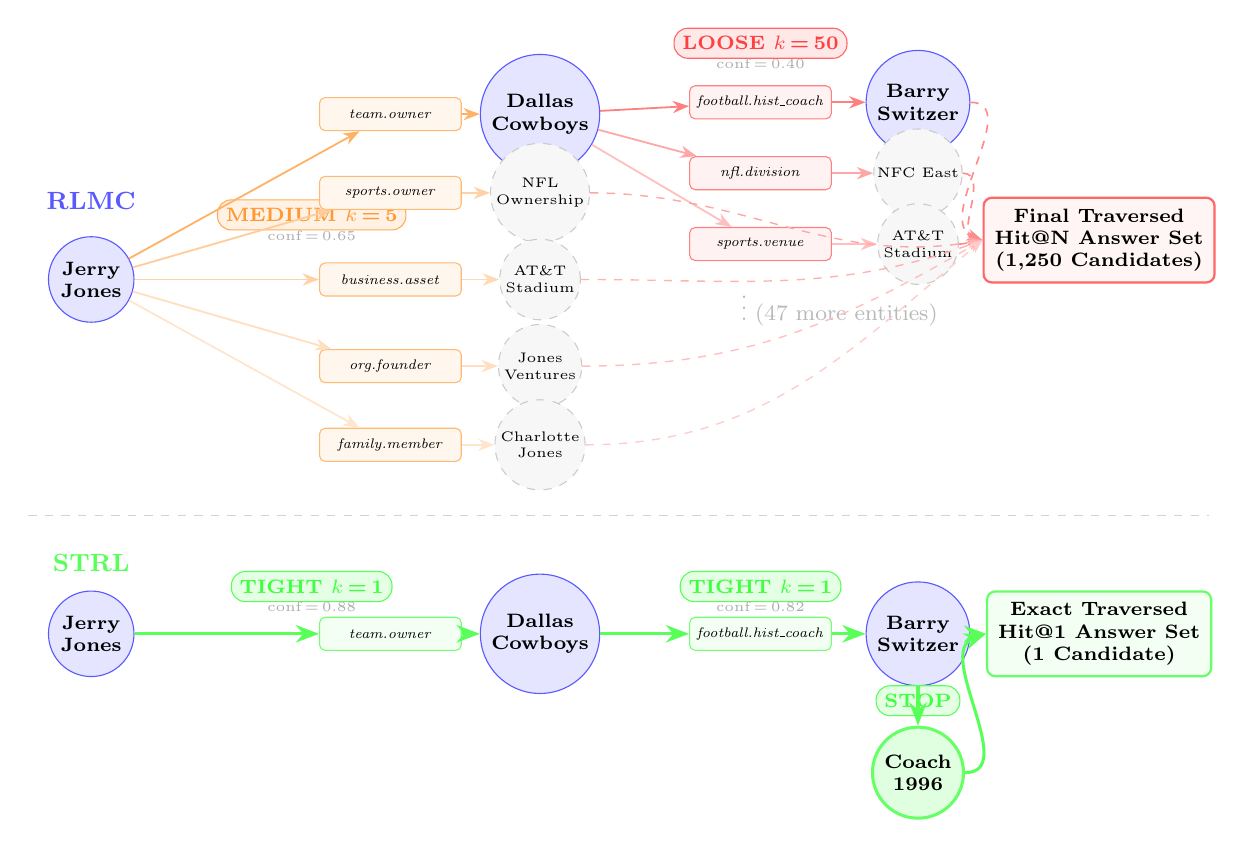
\begin{tikzpicture}[
  font=\small,
  >=Stealth,
  every node/.style={align=center},
  % Entity nodes
  enode/.style={
    circle, draw=blue!65, fill=blue!10,
    inner sep=2pt, minimum size=0.85cm,
    font=\scriptsize\bfseries
  },
  anode/.style={
    circle, draw=green!60, fill=green!12,
    inner sep=2pt, minimum size=0.85cm,
    font=\scriptsize\bfseries, line width=1.1pt
  },
  nnode/.style={
    circle, draw=gray!40, fill=gray!6,
    inner sep=1pt, minimum size=0.75cm,
    font=\tiny, dashed
  },
  % Relation label boxes
  orel/.style={
    rectangle, rounded corners=2pt,
    draw=orange!55, fill=orange!7,
    inner sep=2pt, minimum width=1.8cm, minimum height=0.42cm,
    font=\tiny
  },
  rrel/.style={
    rectangle, rounded corners=2pt,
    draw=red!50, fill=red!5,
    inner sep=2pt, minimum width=1.8cm, minimum height=0.42cm,
    font=\tiny
  },
  grel/.style={
    rectangle, rounded corners=2pt,
    draw=green!55, fill=green!5,
    inner sep=2pt, minimum width=1.8cm, minimum height=0.42cm,
    font=\tiny
  },
  % Action pills
  opill/.style={
    rectangle, rounded corners=5pt,
    draw=orange!65, fill=orange!11,
    inner sep=3pt, font=\scriptsize\bfseries, text=orange!80
  },
  rpill/.style={
    rectangle, rounded corners=5pt,
    draw=red!60, fill=red!9,
    inner sep=3pt, font=\scriptsize\bfseries, text=red!75
  },
  gpill/.style={
    rectangle, rounded corners=5pt,
    draw=green!65, fill=green!10,
    inner sep=3pt, font=\scriptsize\bfseries, text=green!75
  },
  % Arrows
  oarr/.style={->, draw=orange!60, line width=0.65pt},
  rarr/.style={->, draw=red!50, line width=0.65pt},
  Garr/.style={->, draw=green!65, line width=1.2pt},
  mainarr/.style={->, draw=blue!70, line width=1.1pt},
]

% ╔══════════════════════════════════════════════════════════╗
% ║   Standard RL  (MEDIUM at hop1, LOOSE at hop2)          ║
% ╚══════════════════════════════════════════════════════════╝
\node[font=\small\bfseries, text=blue!65] at (0, 1.0) {RLMC};

% Hop 0 entity
\node[enode] (a0) at (0,0) {Jerry\\Jones};

% ── MEDIUM (k=5): 5 relation nodes each ending at entity ──
\node[opill] at (2.8, 0.82) {MEDIUM $k$\,=\,5};
\node[font=\tiny, text=gray!65] at (2.8, 0.56) {conf\,=\,0.65};

% relation + destination pairs (branch out vertically)
\node[orel] (m1r) at (3.8, 2.1)  {\textit{team.owner}};     \node[enode] (m1e) at (5.7, 2.1)  {Dallas\\Cowboys};
\node[orel] (m2r) at (3.8, 1.1)  {\textit{sports.owner}};   \node[nnode] (m2e) at (5.7, 1.1)  {NFL\\Ownership};
\node[orel] (m3r) at (3.8, 0.0)  {\textit{business.asset}}; \node[nnode] (m3e) at (5.7, 0.0)  {AT\&T\\Stadium};
\node[orel] (m4r) at (3.8,-1.1)  {\textit{org.founder}};    \node[nnode] (m4e) at (5.7,-1.1)  {Jones\\Ventures};
\node[orel] (m5r) at (3.8,-2.1)  {\textit{family.member}};  \node[nnode] (m5e) at (5.7,-2.1)  {Charlotte\\Jones};

\draw[oarr] (a0) -- (m1r); \draw[oarr] (m1r) -- (m1e);
\draw[oarr, draw=orange!40] (a0) -- (m2r); \draw[oarr, draw=orange!35] (m2r) -- (m2e);
\draw[oarr, draw=orange!35] (a0) -- (m3r); \draw[oarr, draw=orange!30] (m3r) -- (m3e);
\draw[oarr, draw=orange!25] (a0) -- (m4r); \draw[oarr, draw=orange!25] (m4r) -- (m4e);
\draw[oarr, draw=orange!20] (a0) -- (m5r); \draw[oarr, draw=orange!20] (m5r) -- (m5e);

% ── LOOSE (k=50): from Dallas Cowboys, 3 visible + dots ──
\node[rpill] at (8.5, 3.0) {LOOSE $k$\,=\,50};
\node[font=\tiny, text=gray!65] at (8.5, 2.74) {conf\,=\,0.40};

\node[rrel] (l1r) at (8.5, 2.25)  {\textit{football.hist\_coach}}; \node[enode] (l1e) at (10.5, 2.25) {Barry\\Switzer};
\node[rrel] (l2r) at (8.5, 1.35)  {\textit{nfl.division}};          \node[nnode] (l2e) at (10.5, 1.35) {NFC East};
\node[rrel] (l3r) at (8.5, 0.45)  {\textit{sports.venue}};          \node[nnode] (l3e) at (10.5, 0.45) {AT\&T\\Stadium};
\node[font=\footnotesize, text=gray!55] at (9.5,-0.3) {$\vdots$\ (47 more entities)};

\draw[rarr] (m1e) -- (l1r); \draw[rarr] (l1r) -- (l1e);
\draw[rarr, draw=red!35] (m1e) -- (l2r); \draw[rarr, draw=red!35] (l2r) -- (l2e);
\draw[rarr, draw=red!25] (m1e) -- (l3r); \draw[rarr, draw=red!25] (l3r) -- (l3e);

% ── Massive Noise Candidate Answer Set (Hit@N Candidates) ──
\node[rectangle, rounded corners=3pt, draw=red!60, fill=red!4, font=\scriptsize\bfseries, inner sep=4pt, line width=0.8pt] (cset) at (12.8, 0.5) {Final Traversed\\Hit@N Answer Set\\(1,250 Candidates)};

% Outflow arrows from each traversed node to show they are all collected into Hit@N Candidates set
\draw[->, draw=red!45, dashed, line width=0.6pt] (l1e.east) to[out=0, in=160] (cset.west);
\draw[->, draw=red!45, dashed, line width=0.6pt] (l2e.east) to[out=0, in=170] (cset.west);
\draw[->, draw=red!45, dashed, line width=0.6pt] (l3e.east) to[out=0, in=180] (cset.west);
\draw[->, draw=red!35, dashed, line width=0.5pt] (m2e.east) to[out=0, in=190] (cset.west);
\draw[->, draw=red!30, dashed, line width=0.5pt] (m3e.east) to[out=0, in=200] (cset.west);
\draw[->, draw=red!25, dashed, line width=0.5pt] (m4e.east) to[out=0, in=210] (cset.west);
\draw[->, draw=red!20, dashed, line width=0.5pt] (m5e.east) to[out=0, in=220] (cset.west);

% ══ Divider ══
\draw[gray!35, dashed, line width=0.4pt] (-0.8,-3.0) -- (14.2,-3.0);

% ╔══════════════════════════════════════════════════════════╗
% ║   STRL  (TIGHT at every hop)                            ║
% ╚══════════════════════════════════════════════════════════╝
\node[font=\small\bfseries, text=green!65] at (0,-3.6) {STRL};

\node[enode] (b0) at (0,-4.5) {Jerry\\Jones};

% ── Hop 1 TIGHT ──
\node[gpill] at (2.8,-3.9) {TIGHT $k$\,=\,1};
\node[font=\tiny, text=gray!65] at (2.8,-4.15) {conf\,=\,0.88};
\node[grel] (t1r) at (3.8,-4.5) {\textit{team.owner}};
\node[enode] (t1e) at (5.7,-4.5) {Dallas\\Cowboys};
\draw[Garr] (b0) -- (t1r);
\draw[Garr] (t1r) -- (t1e);

% ── Hop 2 TIGHT ──
\node[gpill] at (8.5,-3.9) {TIGHT $k$\,=\,1};
\node[font=\tiny, text=gray!65] at (8.5,-4.15) {conf\,=\,0.82};
\node[grel] (t2r) at (8.5,-4.5) {\textit{football.hist\_coach}};
\node[enode] (t2e) at (10.5,-4.5) {Barry\\Switzer};
\draw[Garr] (t1e) -- (t2r);
\draw[Garr] (t2r) -- (t2e);

% ── STOP ──
\node[gpill] at (10.5,-5.35) {STOP};
\node[anode, below=0.5cm of t2e] (ans) {Coach\\1996};
\draw[Garr] (t2e) -- (ans);

% ── Exact hit@1 candidate ──
\node[rectangle, rounded corners=3pt, draw=green!60, fill=green!5, font=\scriptsize\bfseries, inner sep=4pt, line width=0.8pt] (gset) at (12.8, -4.5) {Exact Traversed\\Hit@1 Answer Set\\(1 Candidate)};

\draw[->, draw=green!65, line width=1.1pt] (t2e.east) -- (gset.west);
\draw[->, draw=green!65, line width=1.1pt] (ans.east) to[out=0, in=200] (gset.west);

\end{tikzpicture}

\caption{Inference trace on \textit{``Who was the 1996 coach of the team owned by Jerry Jones?''} \textbf{Top (RLMC):} Confidence drops at \textit{Dallas Cowboys}, triggering a \textsc{Loose} action (beam\,=\,50) that expands to 1,250 candidates (dashed noise edges). \textbf{Bottom (STRL):} InfoNCE grounding sustains high confidence at every hop, enabling \textsc{Tight} actions (beam\,=\,1) throughout and reaching the correct answer with exactly 1 candidate. Both pipelines pass candidates to the CDS DPO Judge (F3) for final selection.}
\label{fig:working_example}
\end{figure*}

This trace illustrates the RLMC vs.\ STRL behavioural contrast on the two-hop question \textit{``Who was the 1996 coach of the team owned by Jerry Jones?''} (Jerry Jones $\to$ Dallas Cowboys $\to$ Barry Switzer). Under \textbf{RLMC} (top): the agent selects \textsc{Medium} (beam\,=\,5) at \textit{Jerry Jones}, then encounters high relational density at \textit{Dallas Cowboys}, causing a confidence drop and a \textsc{Loose} action (beam\,=\,50). This avoids missing the correct path (\texttt{football.historical\_coach}) but at significant traversal cost. Under \textbf{STRL} (bottom): InfoNCE grounding keeps representations tightly aligned; the planner maintains confidence $>0.80$ at both hops, enabling \textsc{Tight} actions (beam\,=\,1) that traverse the exact optimal path and trigger \textsc{Stop}, completing with 1 candidate total.

% -----------------------------------------------------------
\section{Ablation Study and Analysis}
\label{app:ablation}
% -----------------------------------------------------------

Since full re-training ablations are computationally prohibitive, we analyze component contributions via observed training dynamics, intermediate checkpoints, and performance trajectory across pipeline configurations.

\subsection{Component Ablations}

\textbf{Without RL Traversal Control.} Replacing adaptive traversal with static fixed-width expansion significantly increases unnecessary graph exploration. The Stage~I-only result (37.2\% Hit@1, Table~\ref{tab:main_results}) confirms that RL-based width control provides a meaningful gain over purely supervised planning.

\textbf{Without Confidence Estimation.} Removing $\eta_q$ destabilizes traversal decisions during ambiguous hops: the controller defaults to expensive \textsc{Loose} actions even when the optimal relation is within a tight beam.

\textbf{Without Decoupled Training.} Jointly optimizing semantic reasoning and traversal during RL leads to unstable simultaneous updates. Freezing Stage~I during Stage~II RL training substantially improves policy stability and convergence speed.

\textbf{Without Semantic Reward Shaping.} Removing InfoNCE supervision causes the agent to exploit graph topology rather than semantic alignment, degrading traversal quality on compositionally ambiguous questions.

\textbf{Without CDS Reranker.} Using raw traversal outputs as final predictions degrades Hit@1 substantially, confirming that path-aware reranking is essential for resolving entity ambiguity after beam expansion.

\subsection{DPO vs.\ SFT-Only Judge}

Replacing the DPO-aligned T5 judge with the SFT-only checkpoint yields a minor $\approx$1\,pp accuracy improvement (41.66\% vs 40.78\%), indicating a slight ``alignment tax'' consistent with known DPO behaviour at small model scales~\cite{rafailov2023direct}. The DPO formulation is nevertheless retained as it directly instantiates RL-family preference alignment at the candidate selection layer—the paper's second RL contribution—ensuring methodological coherence between the traversal-control and selection stages. The marginal accuracy trade-off is accepted in favour of this narrative consistency.

\subsection{Practical Training Challenges}

Several engineering challenges arose that highlight the difficulty of RL over large symbolic KGs:
\begin{itemize}
  \item \textbf{Policy collapse from sparse rewards.} Initializing the RL controller from scratch frequently caused policy collapse; pre-training Stage~I first via supervised objectives was essential for stable RL warm-starting.
  \item \textbf{Traversal explosion.} Early policy iterations expanded tens of thousands of edges per hop in dense Freebase neighborhoods (e.g., high-degree sport/business entities), causing VRAM overflow. Enforcing hard beam caps ($k \le 50$ for \textsc{Loose}) resolved this.
  \item \textbf{Reward sensitivity.} The agent was highly sensitive to $\alpha,\beta,\gamma$ balance. Setting $\alpha$ too high caused the agent to prefer LOOSE regardless of confidence; $\beta$ too high caused premature STOP. Final values were found via grid search on the dev set.
  \item \textbf{Semantic drift without curriculum.} Without the STRL InfoNCE curriculum, the RLMC agent learned to exploit graph topology shortcuts (e.g., high-degree hub nodes reachable via any relation) rather than semantically grounded paths.
  \item \textbf{Windows compatibility constraints.} Training with \texttt{gradient\_checkpointing} and multi-worker dataloaders caused OS paging conflicts on Windows. Setting \texttt{dataloader\_num\_workers=0} resolved stability issues at a minor throughput cost.
\end{itemize}

% -----------------------------------------------------------
\section{Extended Results Analysis}
\label{app:analysis}
% -----------------------------------------------------------

\subsection{Traversal Efficiency}

The TIGHT action (beam\,=\,1) dominates high-confidence hops ($\eta_q > 0.7$), while LOOSE (beam\,=\,50) is primarily triggered at hops where $\eta_q < 0.3$, indicating high semantic ambiguity. Under STRL, the proportion of TIGHT selections increases substantially due to tighter semantic grounding, directly producing the $\sim$14 edges/question result vs.\ $\sim$1,912 under RLMC. This confirms that semantic grounding is the primary driver of traversal efficiency rather than the RL reward signal alone.

\subsection{Effect of Decoupled RL Optimization}

The two-stage decoupled formulation (Stage~I supervised $\to$ Stage~II RL over frozen planner) is key to training stability. In preliminary experiments where both stages were jointly optimized from the start, the RL signal corrupted the planner's cross-hop attention before it could form stable representations, causing policy divergence within 3 epochs. Freezing Stage~I produces a stable semantic manifold over which the compact 4-action policy space can be efficiently explored.

\subsection{Semantic-Guided RL vs.\ Sparse-Only Reward}

The semantic alignment loss $\mathcal{L}_{\text{align}} = 1 - S(z_t, \bar{r}_t)$ penalizes hop projections that diverge from the target relation embedding. Without this signal, the agent learned to select MEDIUM as a universal action (exploiting the moderate accuracy/cost balance), never specializing TIGHT for high-confidence hops or LOOSE for ambiguous ones. Adding semantic alignment immediately improved action diversity and path accuracy.

\subsection{Candidate Disambiguation Analysis}

The gap between Reasoning Recall (63.1\% RLMC, 71.4\% STRL) and Hit@1 (42.1\%, 40.4\%) indicates the CDS pipeline is the primary performance bottleneck. The F1 Fast Filter and F2 Path Ranker are highly effective at noise reduction; the limiting factor is F3 DPO Judge performance when the candidate set is large and contains many semantically similar entities (e.g., multiple people with the same name from different eras). Stronger preference data construction or a cross-encoder F3 with explicit path conditioning would likely close this gap.

\subsection{Reasoning Depth and Stop Prediction}

The adaptive stop mechanism reduces average reasoning depth on single-hop questions from the maximum $H_{\max}=4$ to $\approx$1.3 hops, avoiding unnecessary expansion. For 2-hop questions (the majority of CWQ), average depth is $\approx$2.1 hops, indicating that the stop head correctly identifies terminal states in most cases. Depth accuracy of 65.2\% (RLMC) vs.\ 92.2\% (STRL) shows that tighter semantic grounding also significantly improves stop prediction quality.

% -----------------------------------------------------------
\section{Complexity Analysis}
\label{app:complexity}
% -----------------------------------------------------------

\subsection{Traversal Complexity}

Traditional exhaustive graph traversal operates at $\mathcal{O}(b^{H_{\max}})$ where $b$ is the average branching factor of Freebase ($b \approx 37$ in our subgraph). Adaptive control reduces this to $\mathcal{O}(k^{H_{\max}})$ where $k \in \{5, 10, 50\}$ (inference beam widths) for \textsc{Tight}/\textsc{Medium}/\textsc{Loose}, giving a worst-case reduction of $(37/50)^4$ and a best-case of $(37/5)^4 \approx 3 \times 10^3\times$ for all-TIGHT paths.

\subsection{Planner and Policy Complexity}

The semantic planner applies transformer self-attention over $H_{\max}=4$ latent hop states: $\mathcal{O}(H_{\max}^2 \cdot d_h) = \mathcal{O}(16 \cdot 512)$ per forward pass—negligible compared to graph traversal. The policy head is a 2-layer MLP of fixed size $d_{\text{mlp}}=256$ mapping $\mathbb{R}^{513} \to \mathbb{R}^4$: $\mathcal{O}(1)$ per step. Total inference cost is dominated by LMDB graph lookups and beam expansion, not neural forward passes.

\subsection{CDS Inference Complexity}

F1 (bi-encoder) uses pre-computed entity embeddings: $\mathcal{O}(|\mathcal{B}|)$ cosine lookups. F2 (path ranker) runs one MPNet forward pass per F1 candidate: $\mathcal{O}(200)$ passes. F3 (DPO Judge) runs one T5 forward pass over the concatenated top-15 prompt: $\mathcal{O}(1)$ per question. The CDS pipeline adds a fixed overhead of $\approx$120\,ms/question regardless of $|\mathcal{B}|$.

\end{document}